\documentclass[10pt]{beamer} 
%\usefonttheme{structuresmallcapsserif} 
%% \usepackage{beamerthemeshadow}
\usepackage{verbatim} 
\usetheme{Singapore}
%\usetheme{Pittsburgh}
%\usetheme{Montpellier}
\usepackage{colortbl}
\usepackage{graphicx}
\usepackage{tabularx}
\usepackage[utf8]{inputenc}
\usepackage{listings}
\usepackage{cancel}
\setbeamercolor{alerted text}{fg=lightgray,bg=white}
 \renewcommand{\baselinestretch}{1.5}
     \normalsize
     
% THIS SHOULD BE HERE!
% No unimportant, irrelevant things. Only information.
% Only code if it is of significance.

% get inspired by:
% Simon Jones, Microsoft research, videos.
% John Hughes article How to give a good research presentation.
\title{Towards a Wide-Coverage Grammar for Swedish Using GF}
%\subtitle{\large }
\author{Malin Ahlberg \\ Gothenburg University}
\date{}

\begin{document}
\maketitle

 \begin{frame}
  \frametitle{Grammatical Framework}
  \framesubtitle{Introduction}
  A grammar formalism based on functional programming 
  based on Martin-Löf type theory
  \vspace{5mm}
  \pause
  One abstract grammar \\
  \pause
  One concrete grammar for each language \\
 \end{frame}

 \begin{frame}
  \frametitle{Grammatical Framework}
  \framesubtitle{Resource grammars}
  The resource grammars covers about 20 languages \\
  \vspace{5mm}
  \pause
  Extra module for language specific constructions
 \end{frame}

\begin{frame}
\frametitle{Swedish}
\framesubtitle{} 
\begin{itemize}
\item{Postnominal determination}
\item{Topicalization}
\item{Passive}
\item{Reflexive prononus}
\end{itemize}
\end{frame}

\begin{frame}
\frametitle{The project}
\framesubtitle{} 
Future goal
\begin{itemize}
\item{Grammatical Framework}
\item{SALDO}
\item{Talbanken}
\end{itemize}
\end{frame}



\begin{frame}
\frametitle{The project}
\framesubtitle{} 
Aims 
\begin{itemize}
\item{Grammatical Framework}
\item{SALDO}
\item{Talbanken}
\end{itemize}
\end{frame}



\begin{frame}
\frametitle{A Treebank for GF}
\framesubtitle{} 
Talbanken\\
  \pause
Mapping \\
\end{frame}


\begin{frame}
\frametitle{Mapping}
\framesubtitle{Example} 
\small{\textbf{Talbanken05}}\hspace{160pt}
\small{\textbf{GF abstract tree}}
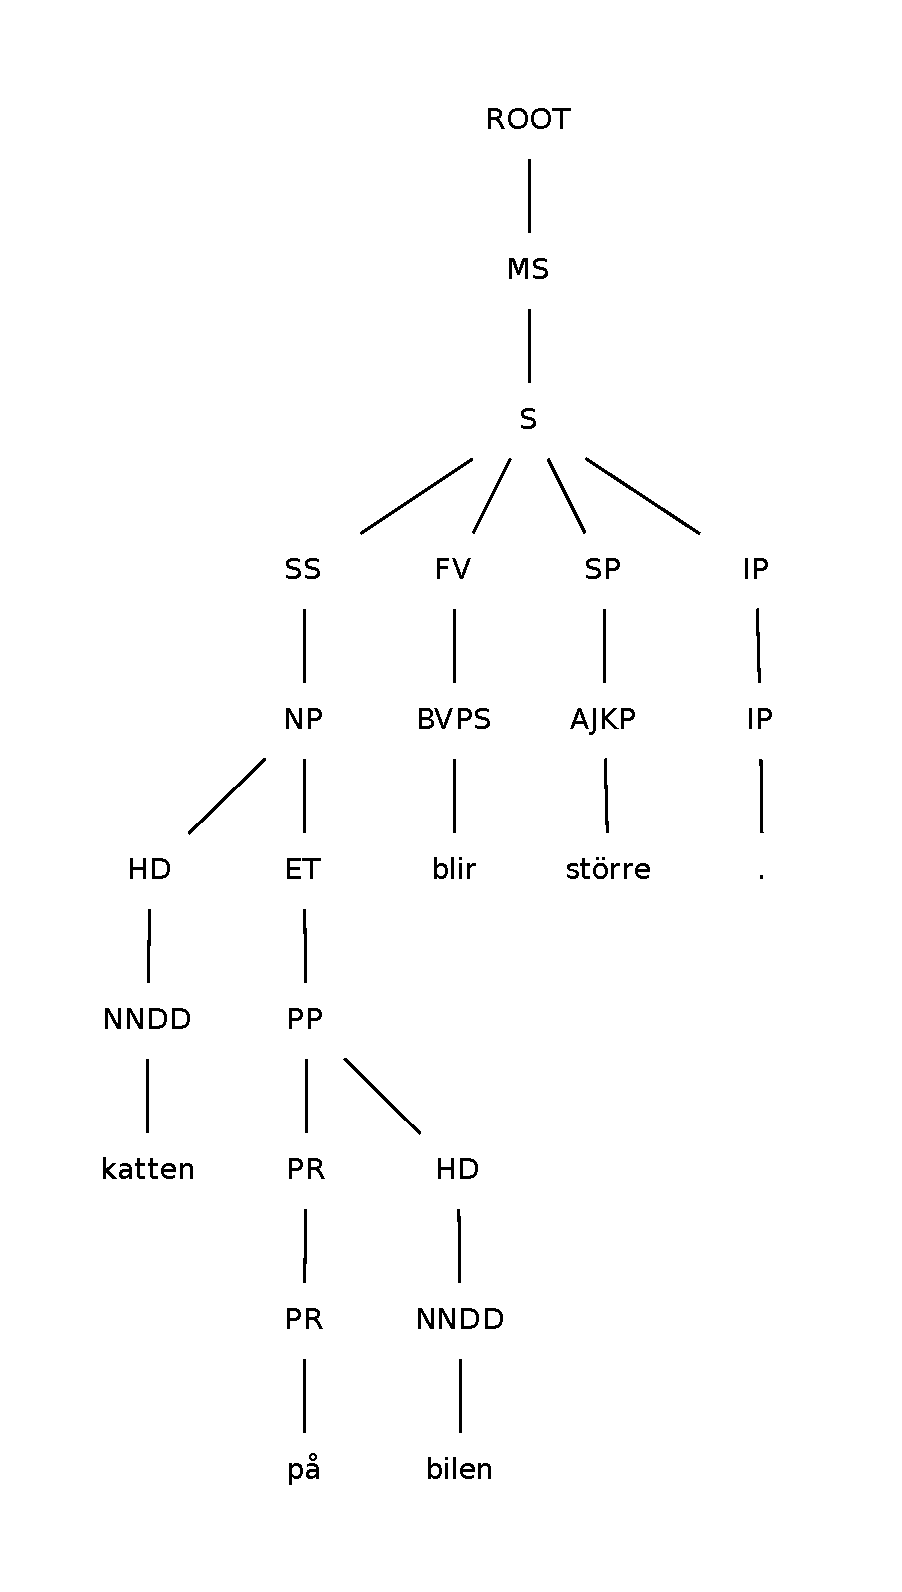
\includegraphics[width=130pt,height=200pt]{taltree.pdf}
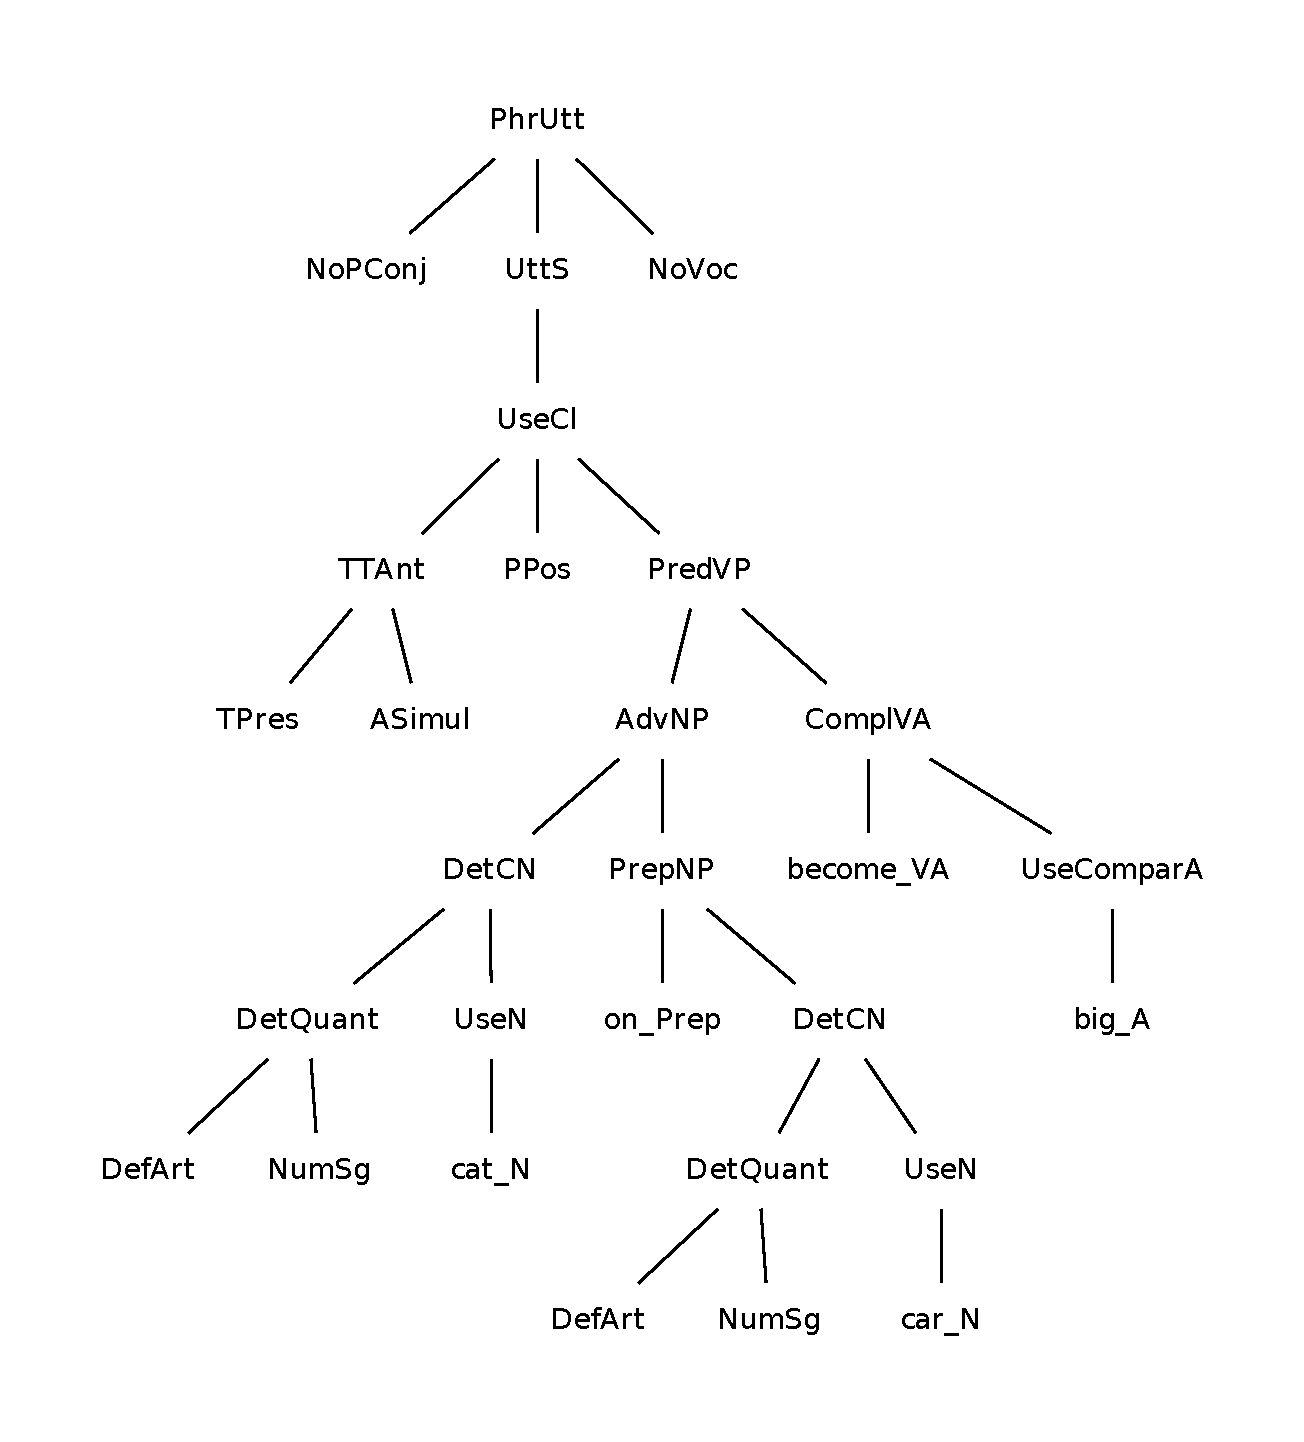
\includegraphics[width=170pt,height=200pt]{gftree.pdf}
\end{frame}

%\begin{frame}
%\frametitle{mapping}
%\framesubtitle{problems} 
%so far 42\% of the easy sentences are totally mapped 
%       10\% not at all
%
%avp
%differnt parsings
%\end{frame}
\begin{frame}

\frametitle{Mapping}
\framesubtitle{Benefits} 
\begin{itemize}
\item{Evaluate the parser}
\pause
\item{Identify grammatical constructions not current in the GF grammar}
\pause
\item{Enable good lexical extraction}
\pause
\item{Extract probabilities for GF functions}
\end{itemize}
% why it's hard (396 hur och hur)
%goals
\end{frame}

\begin{frame}
\frametitle{Mapping}
\framesubtitle{Results} 
% why it's hard (396 hur och hur)
%goals
\end{frame}

\begin{frame}
\frametitle{A large-scale lexicon}
\framesubtitle{Importing Saldo} 
What is saldo \\
picture\\
% why it's hard (396 hur och hur)
%goals
\end{frame}

\begin{frame}
\frametitle{A large-scale lexicon}
\framesubtitle{Importing Saldo} 
The method\\
% why it's hard (396 hur och hur)
%goals
\end{frame}

\begin{frame}
\frametitle{A large-scale lexicon}
\framesubtitle{Results} 
The method\\
Some interesting facts \\
% why it's hard (396 hur och hur)
%goals
\end{frame}

%START OF DEMO
\begin{frame}
\frametitle{The grammar}
\framesubtitle{} 
intersting examples
relate to gullmarsstrand
Passive\\
Formal subjects\\
Topicalisation - with particles, prepositions
Reflexives
\end{frame}

%\begin{frame}
% \renewcommand{\baselinestretch}{1.5}
%\frametitle{The grammar}
%\framesubtitle{Current work} 
%\begin{tabular}{ll}
%\alert{\textbf{ReflGenVP}} & \alert{VPSlash $\rightarrow$ ReflCN $\rightarrow$ VP} \\
%& \alert{\emph{han ger sina små barn till dem}} \\
%{\textbf{PassVP}} & V2 $\rightarrow$ VP \\%  (should be VPSlash $\rightarrow$ VP) \\
%& \emph{äpplet åts} \\ % \;
%\alert{\textbf{AdvVPSlash}} & \alert{VPSlash $\rightarrow$ Adv $\rightarrow$ VPSlash} \\
%& \alert{\emph{hon åt redan äpplet}, \emph{hon är redan här}}\\
%\alert{\textbf{PPartAP}} & \alert{V2 $\rightarrow$ AP} \\
%& \alert{\emph{det är skrivet},\emph{den skrivna artikeln}}
%\end{tabular}\\
%\end{frame}

\begin{frame}
\frametitle{The grammar}
\framesubtitle{Current work} 
\begin{tabular}{ll}
\alert{\textbf{ReflGenVP}} & \alert{VPSlash $\rightarrow$ ReflCN $\rightarrow$ VP} \\
& \alert{\emph{han ger sina små barn till dem}} \\

 %\emph{("äpplet blev ätet")}\\ % boken gavs till honom
\alert{\textbf{PassVP}}
  & \alert{V2 $\rightarrow$ VP} \\ % (should be VPSlash $\rightarrow$ VP)} \\
& \alert{\emph{äpplet åts},}\alert{\emph{boken gavs till honom}} \\ 

% CompAdv here, plus we need ComlVVAdv, Pass? osv
\alert{\textbf{AdvVPSlash}} & \alert{VPSlash $\rightarrow$ Adv $\rightarrow$ VPSlash} \\
& \alert{\emph{hon åt redan äpplet}, \emph{hon är redan här}}\\
% &\emph{("hon åt äpplet redan")} \\

\textbf{PPartAP} & V2 $\rightarrow$ AP \\
& \emph{det är skrivet},\emph{den skrivna artikeln}
\end{tabular}\\
\pause
%Easy sentences with known words (old testsuite) : 92 out of 118 (78\%) \\
%list of functions
%examples
%difficulties
%sådan
\end{frame}

\begin{frame}
 \renewcommand{\baselinestretch}{1.0}
\frametitle{Evaluation}
\framesubtitle{} 
Reached aims
Some nice results
Discussions
\end{frame}



\begin{frame}
 \renewcommand{\baselinestretch}{1.0}
\frametitle{}
\framesubtitle{Future work} 
Lexicon
Probabilitis
Chunk parsing
\end{frame}

\begin{frame}
    \frametitle{The end}
\large\begin{center}Thanks for listening\end{center}
\end{frame}
\end{document}

